\newpage
\section{Playing with Blocks}\label{A:B1}
\index{base-ten blocks} 

I always enjoyed blocks quite a bit. Go find yourself
some \textit{base-ten blocks}. Just so that we are all on the same
page, here are the basic blocks:
\[
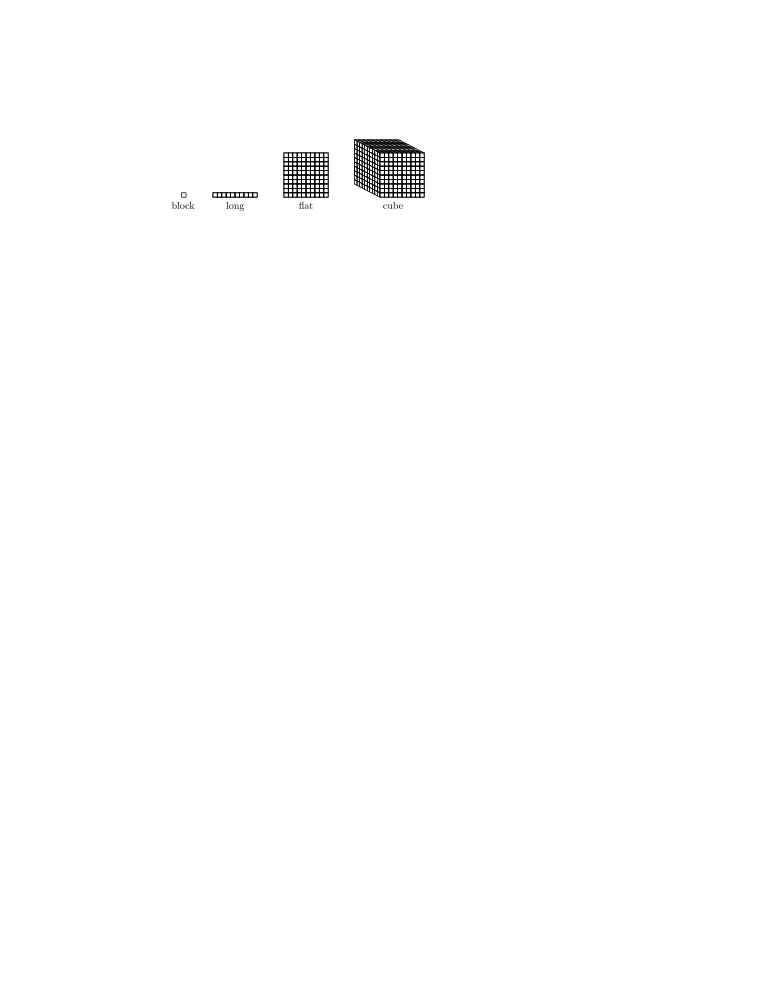
\includegraphics{../graphics/baseTenBlocks.pdf}
\]

\begin{prob} 
Model the number $247$ with base-ten blocks.
\end{prob}

\begin{prob}
Oscar modeled the number $15$ in the following way:
\[
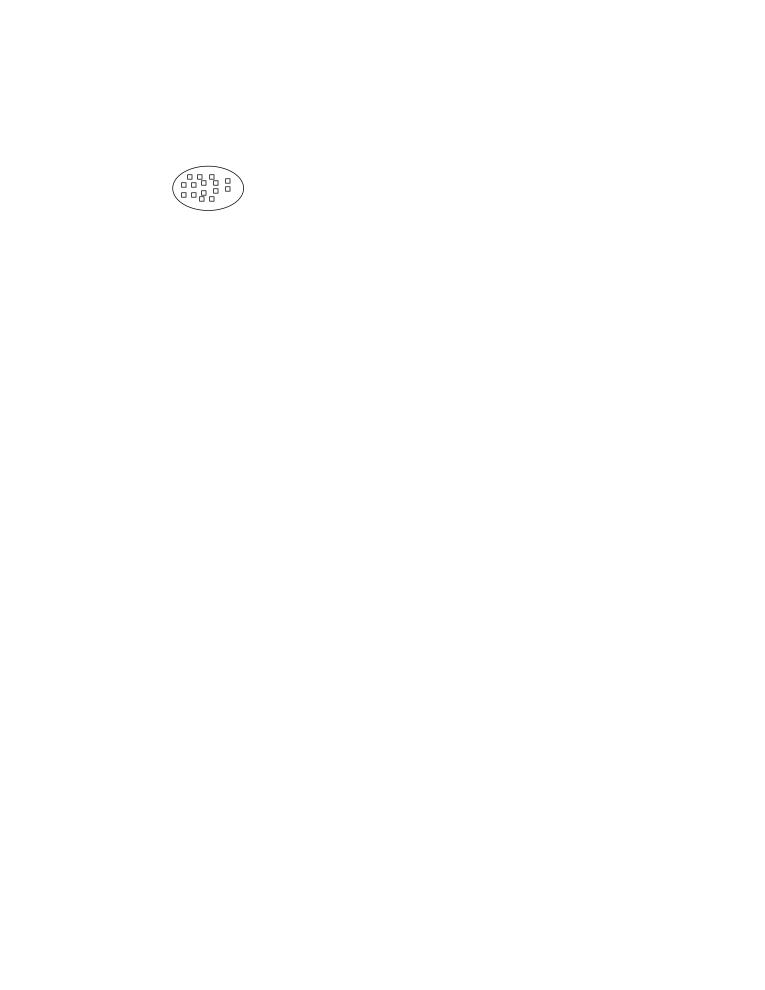
\includegraphics{../graphics/oscarModel.pdf}
\]
What do you think of his model?
\end{prob}

\begin{teachingnote}
The issue here is that the place-value system is not modeled. When
working with base-10 blocks, we will demand that the place value
system is always modeled.
\end{teachingnote}

\fixnote{First ask students to model standard subtraction algorithm, and write the behind the scene's algebra.  Then show Oscar's method and ask the students to write an algorithm showing Oscar's method.}  

\fixnote{Highlight take-away, comparison, and missing addend.}

\newpage

\begin{prob} 
Now Oscar is modeling the basic subtraction
  algorithm:\index{subtraction algorithm!basic}
\[
\begin{tabular}{@{}r@{}r@{}r@{}r@{}}
&   & 8 &  \\
& 8 & $\not{\hspace{-.2ex}9}$ & $\hspace{.3ex}\leftexp{1}2$\\
$-$ & 3 & 7 & 8\\ \hline
& 5 & 1 & 4
\end{tabular}
\]
\[
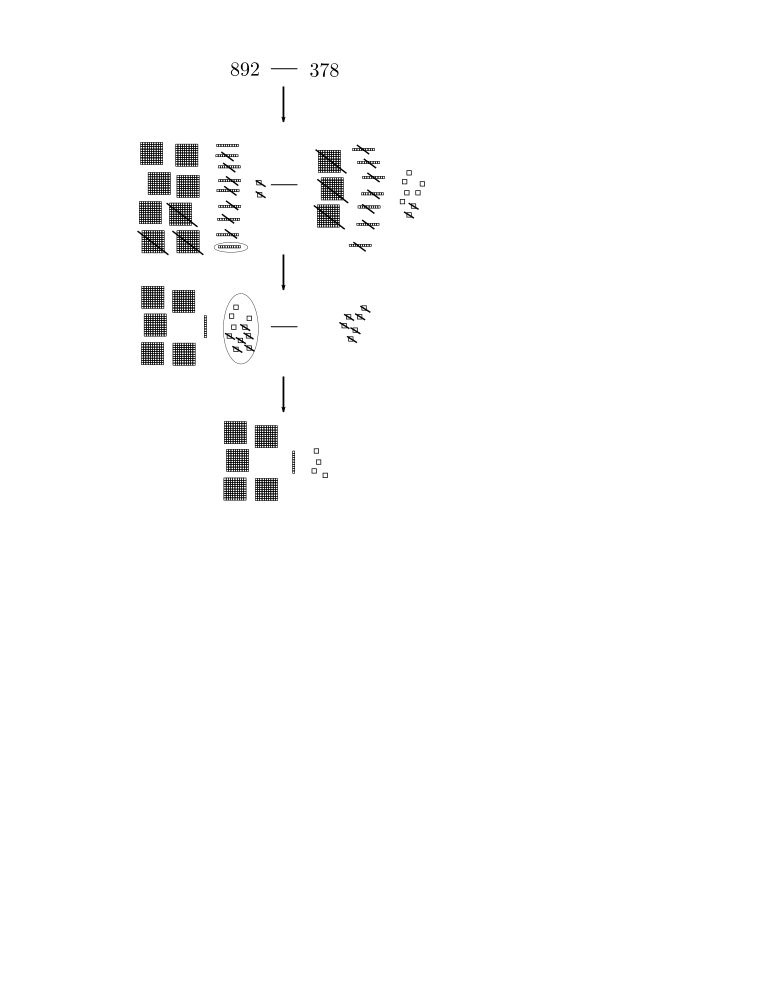
\includegraphics{../graphics/oscarSub.pdf}
\]
Can you explain what is going on? What do you think of his model? Can
you give a better model?
\end{prob}

\begin{teachingnote}
Here the issue is that the actual operations of the algorithm are not modeled.
\end{teachingnote}

\
\begin{prob} Create a ``new'' subtraction algorithm based on Oscar's model.
\end{prob}


\begin{prob}
Here is an example of the basic addition algorithm:
\[
\begin{tabular}{@{}r@{}}
11~~\\
892\\
+398\\ \hline
1290
\end{tabular}
\]
Explain how to model this algorithm with base-ten blocks.
\end{prob}




